\newpage
\part{Project Maker} \label{part:pm}

\section{Introduction to the ProjectMaker module} \label{sec:pmintro}
The \textit{ProjectMaker} module guides through the half-automated assessment of cost-relevant quantities and ecological project benefits. A ``restoration plan'' or project proposal for a restoration plan herein designates an isolated restoration measure in a river \emph{REACH} at a selected site. \emph{version}s of a restoration plan may refer to terraforming options or other planning \emph{condition}s (year). A project proposal is prepared for (preliminarily) definite \emph{version}s of a restoration plan including relevant soil bioengineering restoration features, i.e., vegetation plantings and stabilizing features including the placement of angular boulder and engineered log jams, and it evaluates cost-relevant quantities. A project cost table uses the cost-relevant quantities for a preliminary cost assessment. The habitat utility in terms of net gain in weighted usable habitat (WUA) for target fish species determines the project return in ``US~\$ per [yd$^2$ or m$^2$] of newly created WUA''.\\ 

This chapter explains the module application in the following sections:\\
\begin{tabular}{l L{0.9\textwidth}}
\multicolumn{2}{l}{}\\
Section~\ref{sec:pmquick}: & Application of the GUI with descriptions of input requirements.\\
Section~\ref{sec:pmcq}:  & Generating a project plan and running a cost-quantity assessment with \textit{Project Maker}.\\
Section~\ref{sec:pmmaps}:  & Mapping final designs of features and the construction site.\\
Section~\ref{sec:pmwua}:  & Calculation of WUA and final results.\\
\multicolumn{2}{l}{}\\
\end{tabular}


\section{Quick GUIde to a project assessment} \label{sec:pmquick}
\subsection{Prerequisites}\label{sec:pmprereq}
Ensure that the following steps were executed in order to generate the required geodata for creating a project proposal:
\begin{itemize}
\item If terraforming applies:
  \begin{itemize}
  \item The \emph{REACH{\myUnderscore}SiteName} restoration terraforming plan was verified with 2D hydrodynamic modeling
  \item The \emph{River Architect} package's \emph{ModifyTerrain} module was applied to calculate excavation / fill volumes (for usage, refer to part~\ref{part:mt}).
  \end{itemize}
\item The \emph{LifespanDesign} and \emph{MaxLifespan} modules were executed for plantings and bioengineering features. Thus, the following directories should exist and contain plantings and other bioengineering rasters:
  \begin{itemize}
  \item Plantings:\\
    \texttt{$\ldots{}$/RiverArchitect/MaxLifespan/Products/Rasters/}\\ \texttt{20XX{\myUnderscore}REACH{\myUnderscore}lyr20{\myUnderscore}plants/}
  \item Toolbox and Bioengineering:\\
    \texttt{$\ldots{}$/RiverArchitect/MaxLifespan/Products/Rasters/}\\ \texttt{20XX{\myUnderscore}REACH{\myUnderscore}lyr20{\myUnderscore}toolbox/}
  \end{itemize}
\item The \emph{HabitatEvaluation} module was applied to the pre-project (initial) condition and the "with implementation" condition.
\end{itemize}

\subsection{Main window set-up and run} 
The \textit{ProjectMaker} GUI is shown in Fig.~\ref{fig:gui_start_pm}. The creation of a cost-benefit assessment requires the step-wise definition of variables and calculation beginning at the top of the GUI and moving forward to the bottom. The following sections provide details regarding input requirements and calculations of every step.
\begin{figure}[!h]
	\begin{center}
	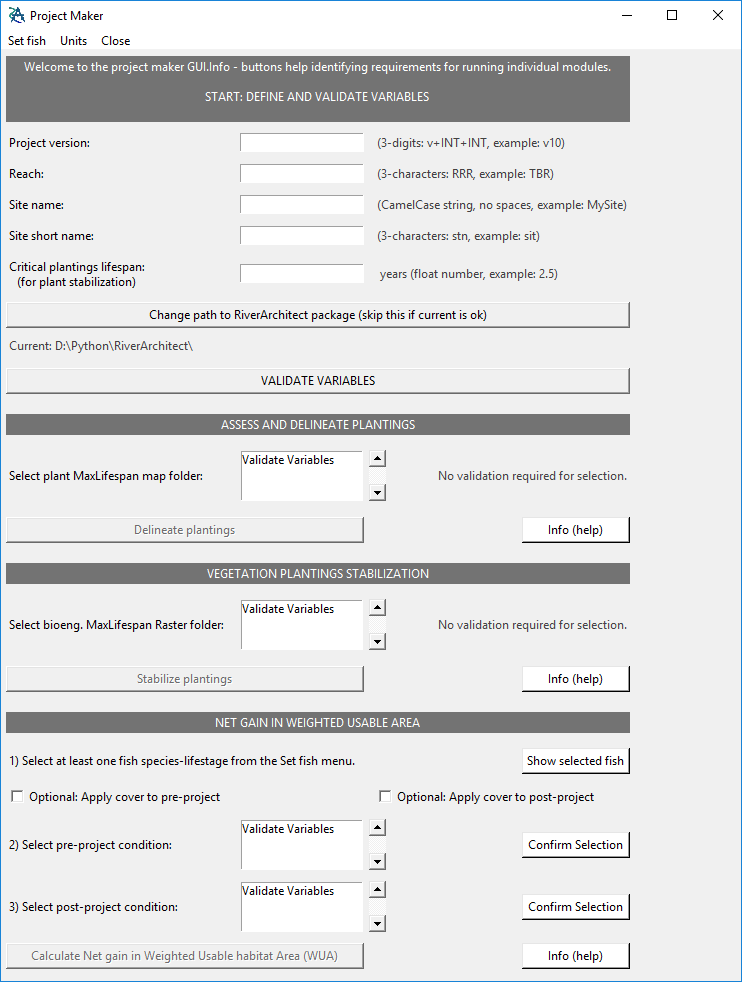
\includegraphics[width=1.0\columnwidth]{gui_start_pm.PNG}
	\caption{GUI start up window. \label{fig:gui_start_pm}}
	\end{center}
\end{figure}

\subsection{Input: Variables and automatically generated files}
The assessment uses the following parameters and formats, which can be entered in the GUI:
\begin{itemize}
  \item \textit{version} (or vii) is a "\textit{v}" + 2-digits (\textit{ii}) version number (string), e.g., \texttt{v10}
  \item \textit{condition} is a 4-digits year indicator (int), e.g., \texttt{2008}
  \item \textit{REACH} is a 3-char reach indicator (string), e.g., \texttt{TBR}
  \item \textit{SiteName} is a site name string written in CamelCase, e.g., \texttt{BigRavine}
  \item \textit{stn} is a 3-char short name string of the site name, e.g., \texttt{rav}
\end{itemize}

Click on the \texttt{VALIDATE VARIABLES} button to verify that the variables entered are correct. A successful validation opens an info-box, a project assessment workbook, and a layout file that invites to create project specific files. The required actions include:

\begin{itemize}
\item WORKBOOK (\emph{REACH}{\myUnderscore}\emph{stn}{\myUnderscore}\emph{costs}{\myUnderscore}\emph{version}.xlsx)\\
	The workbook contains a spreadsheet named \emph{costs}, where unit costs and quantities are evaluated. The \emph{from{\myUnderscore} geodata} spreadsheet will contain quantities such as area (in square meters or acres) of vegetation planting types. The numbers in the \emph{from{\myUnderscore}geodata} tab are generated by a subset of codes that use geodata, which require manual actions as described in the next steps. 
\item LAYOUT FILE\\
  	Save a copy by replacing the project parameters: \emph{REACH}{\myUnderscore}\emph{SiteName}{\myUnderscore}\emph{vii.mxd} and proceed to the creation of required input geodata as described in the next sections.
\end{itemize}

\subsection{Input: Project Area Polygon shapefile} \label{sec:pminp2}
To determine cost-relevant quantities for a site-related restoration plan, a manual delineation of the project site is necessary, e.g., by using the \emph{REACH}{\myUnderscore}\emph{SiteName}{\myUnderscore}\emph{vii.mxd} layout file.

\begin{enumerate}
\def\labelenumi{\arabic{enumi})}
\item Create a new polygon-shapefile in $\ldots{}$\texttt{/Geodata/Shapefiles/} and name it \emph{ProjectArea}.
\item Remove the newly created layer from \emph{mxd} file's \emph{Table of Contents}, double-click on the existing \emph{Project area} layer $\rightarrow$~\emph{Layer Properties} opens up $\rightarrow$~go to the \emph{Source} tab $\rightarrow$~click on \emph{Set Data Source}\ldots{} $\rightarrow$~Select the newly created \texttt{/Shapefiles/}\emph{ProjectArea.shp} file $\rightarrow$~click \emph{OK}.
\item In the \emph{mxd} file's \emph{Table of Contents}, right-click on the \emph{Project area} layer, then \emph{Open Attribute Table}. In the \emph{Table}, click on the top-left drop-down menu and \emph{Add field \ldots{}}. Add a \emph{Text}--type (\emph{length} = 50) field named \emph{AreaCode} and add another \emph{short integer}--type (\emph{precision} = 0) field named \emph{gridcode}. Close the table.
\item  Delineate project area
  \begin{enumerate}
  \def\labelenumii{\alph{enumii}.}
  \item Optional: Import modified terrain to visualize boundaries of terraforming
  \item In the \emph{mxd} file's \emph{Table of Contents}, right-click on the \emph{Project area} layer, then \emph{Edit Features} $\rightarrow$~\emph{Start editing}.
  \item In the \emph{Create Features} tab, click (highlight) on \emph{ProjectArea}, then in \emph{Construction Tools} field, click on \emph{Polygon}.
  \item Draw a polygon around the designated project area (finish with the \emph{F2}-key).
  \item Go to the \emph{Attributes} tab and type \emph{Restoration zone} (\emph{text}) in the \emph{AreaCode} field and \emph{1} (\emph{short integer}) in the \emph{gridcode} field.
  \item Save edits and stop editing.
  \end{enumerate}
\end{enumerate}

\subsection{Input: Delineate Plantings shapefile}\label{sec:pminp3}
The \emph{MaxLifespan} module produces geofiles, i.e., rasters and shapefiles, for complete river reaches. In addition, terraforming may require clearing of existing vegetation in the project area. An overlay of the above created project area polygon over recent satellite image shows, where existing shrubs intersect with projected terraforming surfaces. A \emph{PlantDelineation.shp} shapefile with polygons delineating these intersects needs to be created and drawn as follows in the ...\texttt{/Geodata/\emph{REACH{\myUnderscore}SiteName{\myUnderscore}vii.mxd}}layout file:

\begin{enumerate}
\def\labelenumi{\arabic{enumi})}
\item In the Catalog tab, open the folder tree \ldots{}\texttt{/Geodata/Shapefile} (double click on the folder to make it appear in the lower box).
\item Right-click in the lower box, click on \emph{New} $\rightarrow$~\emph{Shapefile} and name is PlantDelineation (type: \emph{Polygon}); ensure that the coordinate system is coherent with other layers of \emph{REACH{\myUnderscore}SiteName{\myUnderscore}vii.mxd}.
\item Remove the newly created layer from \emph{mxd} file's \emph{Table of Contents}, double-click on the existing \emph{Clearing of shrubs} layer $\rightarrow$~\emph{Layer Properties} opens up $\rightarrow$~go to the \emph{Source} tab $\rightarrow$~click on\emph{Set Data Source}\ldots{} $\rightarrow$~Select the newly created ...\texttt{/Shapefiles/}\emph{PlantDelineation.shp} file $\rightarrow$~click \emph{OK}.
\item In the \emph{mxd} file's \emph{Table of Contents}, right-click on the layer \emph{PlantDelineation}, then \emph{Open Attribute Table}. In the \emph{Table}, click on the top-left drop-down menu and \emph{Add field\ldots{}}. Add a \emph{Text}--type (\emph{length} = 50) field named \emph{ActionType} and add another \emph{short integer}--type (\emph{precision} = 0) field named \emph{gridcode}. Close the table. 
\item Delineate existing plantings area:
  \begin{enumerate}
  \def\labelenumii{\alph{enumii}.}
  \item
    Ensure that a valid background image is linked to the \emph{background} layer (\emph{Layer Properties} $\rightarrow$~\emph{Source} tab).
  \item In the \emph{mxd} file's \emph{Table of Contents}, right-click on the layer \emph{PlantDelineation}, then \emph{Edit Features} $\rightarrow$~\emph{Start editing}  
  \item In the \emph{Create Features} tab, click on \emph{ProjectDelineation}, then in \emph{Construction Tools} window, click on \emph{Polygon}.
  \item Draw polygons around existing plantings that are visible on the background (satellite image) project area, within the zone where the modified DEM rasters indicate terrain modification (finish polygon with the \emph{F2}-key).\\
    \textit{When delineating existing plantings for clearing, remember that in stream restoration and habitat enhancement projects ``clearing'' should limit to the absolutely required minimum.}
  \item Go to the \emph{Attributes} tab and type \emph{Clearing} (\emph{text}) in the \emph{ActionType} field and \emph{1} (\emph{short integer}) in the \emph{gridcode} field.
  \item Once all visible plantings within the terraforming project area are delineated, save the edits and stop editing.
  \end{enumerate}
\end{enumerate}

Save and close \emph{REACH{\myUnderscore}SiteName{\myUnderscore}vii.mxd}.

\section{Cost quantity assessment and the cost master workbook}\label{sec:pmcq}
The \texttt{\emph{REACH}{\myUnderscore}\emph{stn}{\myUnderscore}\emph{costs}{\myUnderscore}\emph{version}.xlsx} is subsequently referred to as the \textbf{\textit{cost master workbook}}. The workbook is automatically generated as a template-copy and it contains two \texttt{cost ...} tabs. \textbf{Important:} As a function of the unit system (U.S. Customary or SI metric), \textbf{only keep the relevant cost worksheet and delete the other one} (see Fig.~\ref{fig:deltab}). \textbf{Rename the retained costs tab to \texttt{costs}}.
%The only action required in the workbook is currently to transfer terraforming volumes from the \textit{ModifyTerrain} module to the \emph{terraforming}{\myUnderscore}\emph{volumes} tab (for details refer to Sec.~\ref{sec:pmterraf}).
\begin{figure}[!h]
	\begin{center}
	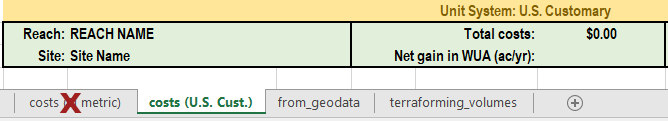
\includegraphics[width=0.75\columnwidth]{deltab.PNG}
	\caption{Delete the non-applicable unit system tab and rename the tab to \texttt{costs}. \label{fig:deltab}}
	\end{center}
\end{figure}

The prices contained in the cost master workbook are in US~$\$$ and may be adapted to fit local construction costs. The following sections describe steps and requirements for the assessment of cost-relevant quantities with the cost master workbook.

\subsection{Terraforming} \label{sec:pmterraf}

The \emph{ModifyTerrain} module evaluated terrain excavation and fill volumes. \emph{ModifyTerrain} created spreadsheets featuring terraforming volumes in cubic meters / yards in the directory \texttt{\ldots{}/RiverArchitect/ModifyTerrain/Output/Spreadsheets/\emph{condition}{\myUnderscore}volumes.xlsx} (see also \ref{part:mt}). Optionally, these workbooks can be copied to a \emph{condition}{\myUnderscore}volumes.xlsx spreadsheet in the project folder.\\

Recall: \emph{condition{\myUnderscore}volumes.xlsx} has to tabs: (1) \emph{excavate{\myUnderscore}YYYYMMDD{\myUnderscore}HHhMM} and (2) \emph{fill{\myUnderscore}YYYYMMDD{\myUnderscore}HHhMM}. Copy the terraforming volumes from either of these two spreadsheets to
the cost master workbook's (\emph{REACH{\myUnderscore}stn{\myUnderscore} costs{\myUnderscore}vii.xlsx}) \emph{terraforming{\myUnderscore}volumes} spreadsheet (cells are highlighted, only values).\\

The template's unit costs of US~\$~10.52 per cubic yard include transport and material storage. It is hypothesized that the smaller value, i.e., either the reach's \emph{excavate} or the reach's \emph{fill} volume, reduces the higher value's costs by half of the unit costs. This assumption is made because the smaller volume can be reused on-site, and therefore, material storage and transport costs reduce. The costs for terraforming works are evaluated in cell \emph{G8} of the \emph{cost} tab of \emph{condition}{\myUnderscore}volumes.xlsx based on the excavate and fill volumes that need to be copied to the \emph{terraforming{\myUnderscore}volumes} tab of \emph{condition}{\myUnderscore}volumes.xlsx. The following formula applies (\emph{vol} refers to the \emph{terraforming{\myUnderscore}volumes} spreadsheet):\\

\(costs!G8 = \ costs!D8 \cdot min(vol!C5,\ \ vol!C6) \cdot \left\lbrack \frac{1}{2} + \left( \frac{max(vol!C5,\ vol!C6)}{min(vol!C5,\ vol!C6)} - 1 \right) \right\rbrack\)



\subsection{Vegetation plantings and supporting features}

Before the most reasonable vegetation plantings are implemented into the project plan, the \emph{MaxLifespan} module needs to be run based on anew 2D simulations made with the terraformed DEM. The resulting maximum lifespan rasters should be available in the directory
\texttt{\ldots{}/RiverArchitect/MaxLifespan/Products/Rasters/\emph{condition}{\myUnderscore}\emph{reach}{\myUnderscore}lyr20{\myUnderscore}plants/} and \texttt{\ldots{}/RiverArchitect/MaxLifespan/Products/}\\\texttt{Rasters/\emph{condition}{\myUnderscore}\emph{reach}{\myUnderscore}lyr20{\myUnderscore}toolbox/}.

\subsubsection{Delineation of most suitable plantings based on maximum lifespan maps} \label{sec:pmactm}

The GUI's \emph{Delineate plantings} button launches a python function that picks up these maximum lifespan rasters, limits there extents to the \emph{ProjectDelineation} Polygon and evaluates relevant quantities for construction purposes. When the calculation has successfully finished, the function's log file (\emph{logfile{\myUnderscore}20.log}) automatically opens. Read the log file carefully and ensure that no error or warning messages occurred. If error messages occurred, check the geodata sources and error messages, ensure that the costs master file (\emph{REACH{\myUnderscore}stn{\myUnderscore}costs{\myUnderscore}vii.xlsx}) is closed and trace back error messages. Re-run \emph{Delineate Plantings} and trace back error messages until no error messages occur anymore.\\

After a successful run, \emph{Delineate plantings} has written vegetation plantings areas to the cost master workbook's \emph{from{\myUnderscore}geodata} spreadsheet. The \emph{costs} spreadsheet automatically evaluates plantings in the \emph{Vegetation plantings}
frame. Nevertheless, double-check assigned cell links to the \emph{from{\myUnderscore}geodata} spreadsheet and close the cost master workbook. \emph{Delineate plantings} saves the cropped maximum lifespan rasters and shapefiles with area summaries in the /Rasters/ and Shapefiles/ subfolders. If the cell links in the automatically opened cost master workbook's \emph{costs} spreadsheet are correct, save and close the workbook.

\subsubsection{Stabilize plantings with low expected lifespan}

Even though the vegetation plantings maximum lifespan maps identify the optimum plantings types according to the highest lifespans, the projected vegetation plantings may be associated with low lifespans. Therefore, supporting (stabilizing) features such as engineered log jams (here: single anchored logs or root wads) may be required. The GUI's \emph{Stabilize plantings} button launches a python function that adds stabilizing bioengineering features such as anchored wood logs to planting areas associated with the user defined ``\emph{Critical plantings lifespan}'' variable. For example, if \emph{Critical plantings lifespan} equals 2.5~years, all plantings that have an equal or smaller expected lifespan of 5~years get assigned the most suitable bioengineering feature. The \emph{Stabilize plantings} function uses the following priorities of stabilizing features:

\begin{enumerate}
\def\labelenumi{\arabic{enumi})}
\item Large wood logs (diameters defined in \texttt{RiverArchitect/LifespanDesign/.templates/}\\
	\emph{threshold{\myUnderscore}values.xlsx}) if their lifespan is higher than \emph{Critical plantings lifespan}.
\item Engineered (anchored) wood logs, where maximum lifespan maps indicate convenient applicability.
\item Vegetation-based bioengineering features (pre-defined in cost master workbook: brush layers; alternatively, fascines or geotextile can be linked from \emph{costs!F30:F33} to \emph{from{\myUnderscore}geodata!C16*\ldots{}}, where the depth to the groundwater does not exceed the threshold values defined in \texttt{RiverArchitect/LifespanDesign/.templates/}\emph{threshold{\myUnderscore}values.xlsx}.
\item Mineral-based bioengineering features (rock paving), where the depth to the ground water table is insufficient for vegetative stabilization and where the terrain is steeper than the threshold values defined in \texttt{RiverArchitect /LifespanDesign/.templates/}\emph{threshold{\myUnderscore}values.xlsx}.
\item Angular boulders where high dimensionless bed shear stress predictions prohibit the utilization of any above feature.
\end{enumerate}


As before, a log file (\emph{logfile{\myUnderscore}21.log}) opens up at the end of the calculation for verification of the calculation process. \emph{Stabilize plantings} writes construction-relevant numbers for vegetation planting stabilization to the cost master workbook's \emph{from{\myUnderscore}geodata} spreadsheet. The \emph{costs} spreadsheet automatically evaluates stabilizing feature quantities in the \emph{Toolbox stabilization} and \emph{Bioengineering (other)} frames. Nevertheless, check the assigned cell links to the \emph{from{\myUnderscore}geodata} spreadsheet and adapt feature types if required. Moreover, \emph{Stabilize plantings} creates a shapefile called (\emph{Plant{\myUnderscore}stab.shp}) in \texttt{\ldots{}/Geodata/Shapefiles/}. After checking the cell links in the automatically opened cost master workbook's \emph{costs} spreadsheet, save and close the workbook.

\subsection{Bioengineering features (other} 

Additional habitat can be created with cover features, i.e., engineering logs jams or root wads, at locations that result from an expert assessment. To implement cover features, open \ldots{}/Geodata/\emph{REACH{\myUnderscore}SiteName{\myUnderscore}vii.mxd} in order to do the following:

\begin{enumerate}
\def\labelenumi{\arabic{enumi})}
\item Create a new polygon-shapefile in .../Geodata/Shapefiles/ and name it \emph{StreamWood}.
\item Remove the newly created \emph{StreamWood} layer from \emph{mxd} file's \emph{Table of Contents}, double-click on the existing \emph{ELJs (Cover habitat)} layer $\rightarrow$~\emph{Layer Properties} opens up $\rightarrow$~go to the \emph{Source} tab $\rightarrow$~ click on \emph{Set Data Source}\ldots{} $\rightarrow$~Select the newly created .../Geodata/Shapefiles/\emph{StreamWood.shp} file $\rightarrow$~click \emph{OK}. 
\item Start editing the \emph{ELJs (Cover habitat)} layer. 
\item Draw engineered log jams and root wads as 10~ft~x~10~ft (3.5~m~x~3.5~m) rectangles.\\
  \emph{\textbf{Design hints}: }\\
  \emph{Engineered log jams and root wads must not be placed in side channels or anabranched sections of the rivers. However, these features can add ``cover'' habitat in backwater zones or reconnected ponds.}\\
  \emph{A save premise is to keep a distance of at least 100 ft (or approximately 30 m) between individual log jams or root wads. To respect the distances, draw a circle with a diameter of 2$\cdot$100 ft (or approximately 2$\cdot$30 m) and place single engineered log jams in the middle of the circles.}
\item Save the edits and stop editing.
\item Write the number of drawn streamwood to the cost master workbook's (\emph{REACH{\myUnderscore}stn{\myUnderscore}costs{\myUnderscore}vii.xlsx}) \emph{costs} spreadsheet (\emph{Bioengineering} frame).
\end{enumerate}

\subsection{Other civil engineering works}

Site access, terrain acquisition or culverts may be required and contribute to the project costs. Satellite images and GIS measurement tools help identifying the required length of new roads or roads that need to be developed.\\ 
The length of new roads can be evaluated, e.g., by drawing paths transferring the path length in yd' or m' (length yard or meter) to the cost master workbook's (\emph{REACH{\myUnderscore}stn{\myUnderscore}costs{\myUnderscore}vii.xlsx}) \emph{costs} spreadsheet (\emph{Civil engineering \& other} frame). For later revision, export the drawn paths to a newly created folder, e.g., .../Geodata/Shapefiles/ as \emph{*.kmz} file.\\
The resulting costs need to be manually entered in the costs master workbook's (\emph{REACH{\myUnderscore}stn{\myUnderscore}costs{\myUnderscore}vii.xlsx}) \emph{costs} spreadsheet (Civil engineering $\&$ other frame).

\subsection{Other costs and remarks}

The final project costs include site mobilization and demobilization as well as unexpected costs and engineering fees at the bottom of the cost master workbook's (\emph{REACH{\myUnderscore}stn{\myUnderscore}costs{\myUnderscore}vii.xlsx}) \emph{costs} spreadsheet. The total costs for the project proposal are summarized at the top of the \emph{costs} spreadsheet.

\section{Mapping of construction elements}\label{sec:pmmaps}

Open \texttt{\ldots{}/Geodata/\emph{REACH}{\myUnderscore}\emph{SiteName}{\myUnderscore}\emph{vii.mxd}} and switch to \emph{Layout View} (\emph{ArcMap} $\rightarrow$~\emph{View} $\rightarrow$~ \emph{Layout View}). Double click on every layer in the \emph{Table of Contents} and define the correct source files (\emph{Source} tab) that result from the above described cost assessment. Relevant shapefile are stored in \texttt{\ldots{}/Geodata/Shapefiles/} and relevant rasters are stored in \texttt{\ldots{}/Geodata/Rasters/}. Export the map (\emph{ArcMap} $\rightarrow$~\emph{File} $\rightarrow$~\emph{Export Map\ldots{}} ) to the project folder and name it \emph{REACH{\myUnderscore}SiteName{\myUnderscore}vii{\myUnderscore}lyr2x.pdf} (proposition for consistent file naming).


\section{Ecological benefit asessment (Calculate WUA)}\label{sec:pmwua}

The project costs are vetted against the net gain in weighted usable habitat area for target fish species. The GUI's \emph{Calculate Net \textbf{W}eighted \textbf{U}sable habitat \textbf{A}rea} routine calculates usable habitat from rasters that indicate where the Composite Habitat Suitability Index (CHSI) is higher than a selected threshold value.

\subsection{Additional input and requirements}
Every CHSI raster refers to a steady discharge within a flow duration curve. The expected flow exceedance duration per discharge bin multiplied with the usable habitat area is summed up to the WUA. The comparison of the existing (pre-project) and the "with implementation" (post-project) habitat suitability requires the following:

\begin{itemize}
\item
  Both situations (pre- and post-project) were simulated in the 2D hydrodynamic model.
\item
  Flow duration curves for the project site were established (also refer to Sec.~\ref{sec:heintro}):
  \begin{itemize}
  \item
    A workbook template for flow duration curves is available in \texttt{RiverArchitect/HabitatEvalu ation/FlowDurationCurves/flow{\myUnderscore}duration{\myUnderscore}templates.xlsx}
  \item
    The \texttt{Tools} -- folder contains the \emph{make{\myUnderscore}flow{\myUnderscore}duration.py} script that analyses discharge series (mean daily discharge) of any length for producing the required format for WUA calculation. An example file of mean daily discharges for creating a flow duration curve with \emph{make{\myUnderscore}flow{\myUnderscore}duration.py} is provided.
  \end{itemize}
\item
  The \emph{River Architect}'s \emph{HabitatEvaluation} module was executed for both situations (pre- and post-project) to obtain CHSI maps.
\item Example:
  \begin{itemize}
  \item The pre-project terrain DEM dates from 2008 and terrain modifications were performed based on the 2008 DEM in a reach called \texttt{rea}.
  \item Both DEMs, original and modified correspond to pre- and post-project conditions, respectively.
  \item Both DEMs were simulated in the 2D hydrodynamic model with discharges of 100, 200, 500, 1000, 2000, and 5000~cfs (or m$^3$/s).
  \item The corresponding modelling results (flow depth and velocity) were stored in the directories \texttt{RiverArc hitect/01{\myUnderscore}Conditions/2008 and RiverArchitect/01{\myUnderscore}Conditions/2008{\myUnderscore}}\\
  \texttt{rea{\myUnderscore}lyr10}, respectively. The string \texttt{lyr10} refers to terraforming according to the code naming conventions.
  \item The \emph{River Architect}'s \emph{HabitatEvaluation} module applied to both situations with a CHSI threshold value of, e.g., 0.4. This threshold value means that all pixels with a CHSI value lower than 0.4 were considered as being non-habitat and the \emph{HabitatEvaluation} module excludes these pixels from the CHSI rasters. Thus, the \emph{HabitatEvaluation} module produced CHSI rasters that are stored in:
    \begin{itemize}
    \item \texttt{RiverArchitect/HabitatEvaluation/WUA/Rasters/2008} (existing / pre-project)
    \item \texttt{RiverArchitect/HabitatEvaluation/WUA/Rasters/2008{\myUnderscore}rea{\myUnderscore}lyr10} (with implementation / post-project)
    \end{itemize}
  \item Te \emph{HabitatEvaluation} module associated (relative) discharge duration and usable habitat areas with the rasters. For example, if the target fish species was Chinook salmon, juvenile lifestage (naming convention chj), the \emph{HabitatEvaluation} module wrote the usable habitat area and discharge duration to the following workbooks:
    \begin{itemize}
    \item \texttt{RiverArchitect/HabitatEvaluation/WUA/2008{\myUnderscore}chj.xlsx}
    \item \texttt{RiverArchitect/HabitatEvaluation/WUA/2008{\myUnderscore}rea{\myUnderscore}lyr10{\myUnderscore}chj.xlsx}
    \end{itemize}
  \end{itemize}
\end{itemize}

\subsection{Run WUA calculation}
When the above requirements are fulfilled, the \emph{Project Proposal} GUI can assess the difference in usable habitat area between both situations (pre- and post-project), i.e., the net gain in WUA. For starting the calculation, define the above-described input data and confirm the calculation:
\begin{itemize}
\item Select a fish species corresponding to the one analyzed with the \emph{HabitatEvaluation} module, e.g., Chinook salmon, juvenile lifestage. The \emph{Select fish} button turns green after selecting a target fish species + lifestage.
\item Select an initial condition (pre-project) and confirm the selection (button turns green after selection).
\item Select a condition after terraforming (with implementation / post-project) and confirm the selection (button turns green after selection.
\item Click on the \emph{Calculate Net gain in Weighted Usable habitat Area (WUA)} button to start the assessment.
\end{itemize}

The program will run in the background and prompts the calculation progress in the console window.

\subsection{Output}
After a successful run, a copy of the \textbf{cost master workbook} with the file name extension corresponding to the target fish automatically opens. For example, if the target fish was Chinook salmon -- juvenile, the copy of the workbook is \ldots{}\texttt{/REACH\emph{{\myUnderscore}}stn\emph{{\myUnderscore}assessment{\myUnderscore}v}ii\emph{{\myUnderscore}chj.xlsx}}.\\

Moreover, the particular \textbf{usable areas associated with the available discharges were written} to \texttt{/Geodata/\emph{WUA{\myUnderscore}evaluation{\myUnderscore}chj.xlsx}}.\\

The discharge-related \textbf{shapefiles} with polygons of usable habitat area were saved as: \texttt{/Geodata/Rasters/\emph{con dition}/\emph{no}{\myUnderscore}cover/NUM\emph{wua{\myUnderscore}eval.shp}}. NUM is an automatically prefix added by the WUA evaluation routine. The association of the NUM shapefile with the corresponding discharge was logged to: \texttt{/Geodata/\emph{logfile{\myUnderscore}40.log}}.\\

The cells \emph{G3} and \emph{I2/3} in \texttt{REACH\emph{{\myUnderscore}}stn\emph{{\myUnderscore}assessment{\myUnderscore}v}ii\emph{{\myUnderscore}fish.xlsx}}. state the
net gain in WUA and the project return in units of US~\$ per square yard (or m$^2$ for any currency defined) net gain in WUA (comparison of pre- and post-project condition), respectively.


 

